\section{Cache hierarchies, movement, and distributed serving}
\label{sec:hierarchy}
\subsection{A cache hit is a location-dependent event}
A prefix can be present on the destination GPU, retained in host memory, stored
on local SSD, or available at another machine. These cases all avoid some
recomputation but have different latency and resource costs. A remote hit may
be slower than local recomputation. A GPU hit may still wait behind another
request. A cache metadata hit is not proof that the tensors are ready for an
attention kernel.

For cache payload $M$, a useful restore model is
\begin{equation}
 t_{\mathrm{restore}}=t_{\mathrm{lookup}}+t_{\mathrm{queue}}+
 t_{\mathrm{setup}}+\frac{M}{B_{\mathrm{effective}}}+t_{\mathrm{layout}}+
 t_{\mathrm{sync}}.
 \label{eq:restore}
\end{equation}
The terms include object lookup, waiting for IO resources, transfer setup,
effective bandwidth, tensor layout conversion, and synchronization. Multiple
hops may overlap or serialize. Bottleneck link bandwidth is an optimistic
starting point, not necessarily the end-to-end rate. A distributed service must
also reserve destination capacity before advertising completed placement.

\fig{hierarchy}{0.86}{A conceptual KV hierarchy. Storage tiers hold reusable
state; the inference engine owns the state required for active attention.
Metadata/control paths are dashed. Product-specific tier names are not universal:
SGLang HiCache and LMCache use different L1/L2 terminology.}{hierarchy}

\paragraph{Restore versus recompute.}
A local decision compares completion costs, not merely existence:
\begin{equation}
 t_{\mathrm{restore}}+\Delta t_{\mathrm{interference}}
 < t_{\mathrm{recompute}}+\Delta t_{\mathrm{alternative\ queue}}.
 \label{eq:break-even}
\end{equation}
The extra terms matter when restores congest a link or recomputation occupies a
GPU that could serve other requests. For illustration, transferring 1 GiB at
25 GiB/s takes 40 ms before overhead; at 8 GiB/s it takes 125 ms. If fixed
overhead is 1 ms and recomputation costs 150 ms, both may help in isolation.
At 2 GiB, the slower path is already 251 ms. These rates and the recomputation
cost are assumptions, not device specifications or measurements.

\fig{transfer}{0.91}{Analytical restore-time curves from Equation~\ref{eq:restore}
with all terms except setup and transfer set to zero. The horizontal line is an
assumed recomputation cost. Queueing or layout conversion moves the crossover.}{transfer}

\subsection{LMCache: externalizing reusable inference state}
LMCache provides a cache layer that extracts, retains, retrieves, and exchanges
KV state around inference engines. Its technical report describes reuse across
requests and engines, prefill/decode transfers, batched movement, IO/compute
pipelining, and control APIs~\cite{lmcache}. It is not an LLM, tokenizer, or
replacement for the engine's attention scheduler. External cache capacity is
useful only if the correct state can be retrieved at a cost lower than the
alternative.

\begin{figure}[htbp]
\centering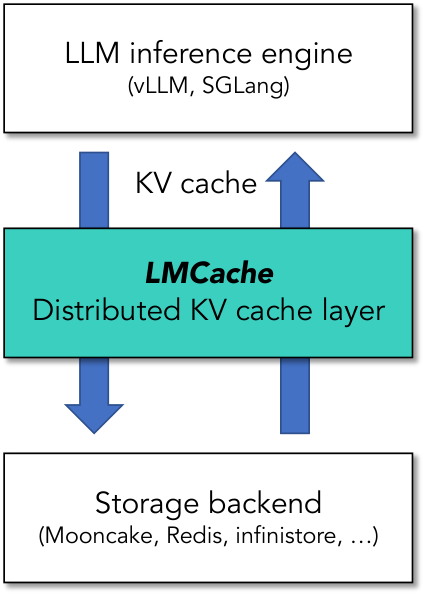
\includegraphics[width=0.52\linewidth]{figures/papers/lmcache.png}
\caption{LMCache's technical-report architecture connects inference engines to
storage and transport backends. Reproduced from Liu et al.~\cite{lmcache},
Figure 5, arXiv:2510.09665v2, CC BY 4.0; scaled only. This depicts the report's
architecture; the current multiprocess implementation is discussed below.}
\label{fig:lmcache-original}
\end{figure}

The current multiprocess architecture documentation places cache management in
a separate server. A storage manager composes local memory management, secondary
storage adapters, and asynchronous store, prefetch, and eviction controllers.
The documented local manager can be backed by CPU DRAM or a GPU-direct-storage
NVMe slab~\cite{lmp}. Therefore describing every LMCache deployment as ``a
Python dictionary of CPU tensors inside vLLM'' is both incomplete and stale.
A deployment must specify its mode, cache ownership, transport, storage backend,
and connector versions.

A conceptual read path is: identify a reusable prefix; discover available
objects; obtain valid access/retention while transferring them; populate the
engine's expected representation; wait for readiness at the required layer or
batch boundary; compute the unmatched suffix. A write path must decide when
and how much completed state to retain. These are generic correctness steps,
not a claim that a particular LMCache release exposes one API per step.

\paragraph{The integration contract that ATFM must verify.}
The legacy in-process controller page is now explicitly deprecated in favor of
multiprocess mode~\cite{llegacy}. Its pin API identifies tokens, an instance,
and a storage location, returning an operation event identifier; the documented
example pins a CPU backend~\cite{lpin}. That does not establish an engine-HBM
reservation, nor does an accepted asynchronous operation prove transfer
completion. ATFM's current HTTP adapter uses older controller-shaped operations
and configurable location strings. Real-worker compatibility is an open
integration task, not something its mock HTTP tests settle.

To make a placement claim defensible, record the engine and connector versions,
resolve session/prompt identity to exact token/cache identity, verify the
supported location, observe operation completion, and check subsequent reuse.
If only a host copy is protected, the expected benefit is avoiding a deeper
reload or recomputation, not guaranteed zero-copy GPU reuse. This distinction
belongs in both experiments and user-facing descriptions.

\subsection{Other cache hierarchies and advanced reuse}
SGLang HiCache organizes GPU, host, and external storage as a hierarchy. Its
radix metadata tracks local state, with backend lookup for external storage;
matching, prefetch, and write-back are separate operations. The documented
prefetch policies trade waiting for reuse against proceeding with available
state~\cite{hicache}. A forecasting controller must compare against these
existing policies, not against an engine with all offloading disabled.

CacheGen compresses KV representations and adapts context loading to network
conditions~\cite{cachegen}. Compression exchanges encoding/decoding and possible
quality costs for fewer bytes. The relevant break-even expression becomes
$t_{\mathrm{encode}}+M_{\mathrm{compressed}}/B+t_{\mathrm{decode}}$, with any
quality restriction treated as a constraint. It is not enough to report the
compression ratio.

CacheBlend addresses reusable passages that are not an identical prefix by
selectively recomputing part of the cached state to account for their new
context~\cite{cacheblend}. This is more involved than concatenating cached
arrays. Changing preceding tokens changes causal representations. A serving
experiment using such reuse must state the method and test output quality,
instead of assuming ordinary exact-prefix semantics.

Tutti, a 2026 preprint, explores a GPU-centric object/IO path for SSD-backed KV
restoration, reducing CPU involvement in critical IO operations~\cite{tutti}.
AsymCache, another 2026 preprint, links eviction and partial-context reuse to
attention-kernel costs rather than maximizing cache hit rate alone~\cite{asym}.
Their relevance here is architectural: transfer orchestration and the location
of missing tokens can matter as much as the count of missing bytes. Their
reported speedups are not reproduced in this paper.

\subsection{Prefill/decode disaggregation}
A colocated engine executes both phases on the same worker group. A
disaggregated system uses separate prefill and decode pools and transfers the
required state between them. DistServe motivates this separation through
independent phase SLOs, resource allocation, and parallelism plans, while
accounting for transfer bandwidth~\cite{distserve}.

\fig{papers/distserve}{1.0}{DistServe's runtime architecture. The global
scheduler coordinates separate prefill and decode worker groups; KV transfer
connects their execution. Reproduced from Zhong et al.~\cite{distserve},
Figure 6, arXiv:2401.09670v3, CC BY-SA 4.0; scaled and format-converted only.}{pd}

The benefit is conditional. Let $\Delta t_{\mathrm{interference}}$ be the
colocation penalty removed and $\Delta t_{\mathrm{specialization}}$ the gain
from better phase-specific allocation. Disaggregation helps a latency objective
only when those gains exceed transfer, extra queueing, and orchestration costs
for the relevant request distribution. It can reduce tail ITL while leaving
aggregate tokens/s unchanged or lower. The versioned vLLM disaggregation guide
frames the feature around separate TTFT/ITL tuning and connector-based
transfer, and labels it experimental in that version~\cite{vdisagg}.

A necessary average transfer-capacity condition is
\begin{equation}
 \lambda_{pd}\E[M_{pd}] < B_{pd,\mathrm{usable}},
\end{equation}
where $\lambda_{pd}$ is transferred requests per second. Even below this bound,
burstiness and concurrent traffic can produce long transfer queues. With several
links and routes, enforce the condition per bottleneck resource; adding all link
bandwidths is invalid when transfers share a narrow hop. More prefill GPUs do
not fix a saturated transfer fabric.

Mooncake's KV-centric architecture combines phase separation with a distributed
cache using other cluster memory/storage resources, and considers overload
handling rather than assuming every arrival can be served~\cite{mooncake}.
This is directly relevant to ATFM: cache, queueing, and admission already interact
in prior systems. The proposed distinction must be the information used and the
validated decision improvement.

\subsection{Routing: reuse versus load}
Routing all related prompts to one worker maximizes locality but may create a
hot spot. Sending them to the shortest queue may discard valuable state. A
conceptual score for destination $j$ is
\begin{equation}
 C_j = \widehat q_j + \widehat t_{\mathrm{missing\ prefill},j}
       +\widehat t_{\mathrm{restore},j}+\widehat t_{\mathrm{decode},j}
       +\widehat c_{\mathrm{risk},j}.
 \label{eq:routing}
\end{equation}
All terms must have consistent units or explicit objective weights. Cache-hit
fraction by itself is not a completion-time score. For example, a 95\% hit with
one second of queueing can lose to a 50\% hit with 100 ms of extra prefill on an
idle worker. This is a constructed illustration, not a measured threshold.
Preble studies the joint optimization of distributed prompt reuse and load
balancing~\cite{preble}.

NVIDIA Dynamo separates frontend handling, worker routing, execution, event
feedback, and scaling/actuation. Its architecture includes backend-specific
transfer coordination~\cite{dynamo}. Its KV-aware routing documentation
explicitly combines reusable cache state with projected active load, and
separates selecting workers from moving their tensors~\cite{drouter}. Its
planner already supports load-based and predictive scaling paths with
aggregate traffic predictors~\cite{dplanner}. ATFM cannot claim that serving
systems only react or never forecast.

llm-d offers a Kubernetes-oriented composition of a gateway proxy, Endpoint
Picker, inference pools, and model servers. The documented architecture includes
cache-aware routing, cache indexing/offload, and disaggregated
serving~\cite{llmd}. It is a deployment/control framework, whereas vLLM is an
engine and LMCache is a cache layer. These components can compose; they are not
three mutually exclusive answers to the same question.

\subsection{State correctness and operational costs}
KV state is derived but sensitive. It can encode information from user input,
so cache sharing needs tenant isolation and authorization in addition to a
collision-resistant identity scheme. A stale location record may cause a miss;
a wrong identity may cause an incorrect answer. Those failure modes deserve
different treatment. Reference counts, leases, transfer completion, and
invalidation must agree with engine ownership.

The costs of a cache policy include background writes, duplicate replicas,
reserved host memory, network congestion, and abandoned prefetched data. A
cache hit-rate improvement can be economically negative if it costs more
resources than it saves. Similarly, a ``touch'' request that refreshes recency
uses frontend and engine capacity and can perturb scheduling. It is a heuristic
actuator, not a free, universal pin primitive.

\takeaway{The decision is not simply whether KV exists. It is whether compatible
state can be made ready at the right worker, before it is needed, at an acceptable
cost to other work. ATFM's forecasts would have to improve that decision beyond
native cache and routing mechanisms.}
